\documentclass[UTF-8,twoside,cs4size]{ctexart}
\usepackage[dvipsnames]{xcolor}
\usepackage{amsmath}
\usepackage{amssymb}
\usepackage{geometry}
\usepackage{setspace}
\usepackage{xeCJK}
\usepackage{ulem}
\usepackage{pstricks}
\usepackage{pstricks-add}
\usepackage{bm}
\usepackage{mathtools}
\usepackage{breqn}
\usepackage{mathrsfs}
\usepackage{esint}
\usepackage{textcomp}
\usepackage{upgreek}
\usepackage{pifont}
\usepackage{tikz}
\usepackage{circuitikz}
\usepackage{caption}
\usepackage{tabularx}
\usepackage{array}
\newcolumntype{Y}{>{\centering\arraybackslash}X}
\usepackage{pgfplots}
\usepackage{multirow}
\usepackage{pgfplotstable}
\usepackage{mhchem}
\usepackage{physics} % Add this package for \dt and \dif commands
\usepackage{cases}
\usepackage{subfigure}
\usepackage{enumerate}
\usepackage{minipage-marginpar}
\usepackage{diagbox}

\graphicspath{{./figure/}}

\setCJKfamilyfont{zhsong}[AutoFakeBold = {5.6}]{STSong}
\newcommand*{\song}{\CJKfamily{zhsong}}

\geometry{a4paper,left=2cm,right=2cm,top=0.75cm,bottom=2.54cm}

\newcommand{\experiName}{微波布拉格衍射}%实验名称
\newcommand{\supervisor}{易栖如}%指导教师
\newcommand{\name}{孙奕飞}
\newcommand{\studentNum}{2023k8009925001}
\newcommand{\class}{2}%班级
\newcommand{\group}{06}%组
\newcommand{\seat}{01}%座位号
\newcommand{\dateYear}{2024}
\newcommand{\dateMonth}{11}%月
\newcommand{\dateDay}{5}%日
\newcommand{\room}{教717}%地点
\newcommand{\others}{$\square$}

\ctexset{
    section={
        format+=\raggedright\song\large
    },
    subsection={
        name={\quad,.}
    },
    subsubsection={
        name={\qquad,.}
    }
}

\begin{document}
\noindent

\begin{center}

    \textbf{\song \zihao{-2} \ziju{0.5}《基础物理实验》实验报告}
    
\end{center}


\begin{center}
    \kaishu \zihao{5}
    \noindent \emph{实验名称}\underline{\makebox[28em][c]{\experiName}}
    \emph{指导教师}\underline{\makebox[9em][c]{\supervisor}}\\
    \emph{姓名}\underline{\makebox[6em][c]{\name}} 
    \emph{学号}\underline{\makebox[14em][c]{\studentNum}}
    \emph{分班分组及座号} \underline{\makebox[5em][c]{\class \ -\ \group \ -\ \seat }\emph{号}} \\
    \emph{实验日期} \underline{\makebox[3em][c]{\dateYear}} \emph{年}
    \underline{\makebox[2em][c]{\dateMonth}}\emph{月}
    \underline{\makebox[2em][c]{\dateDay}}\emph{日}
    \emph{实验地点}\underline{{\makebox[4em][c]\room}}
    \emph{调课/补课} \underline{\makebox[3em][c]{否}}
    \emph{成绩评定} \underline{\hspace{8em}}
    {\noindent}
    \rule[5pt]{17.7cm}{0.2em}
\end{center}

\section{实验目的}
    1.了解与学习微波产生的基本原理及传播和接受等基本特征\par
    2.观察微波衍射、干涉等实验现象\par
    3.观察模拟晶体的微波布拉格衍射现象\par
    4.通过迈克尔逊实验测量微波波长

\section{实验仪器}
DHMS-1 型微波光学综合实验仪一套(图 1),包括:X 波段微波信号源、微波发生器、发
射喇叭、接收喇叭、微波检波器、检波信号数字显示器、可旋转载物平台和支架,以及实验用附
件(反射板、分束板、单缝板、双缝板、晶体模型、读数机构等)。

\section{实验原理}
\subsection{综述}
微波的波长范围从 $1\,\mathrm{m}$ 到 $0.1\,\mathrm{mm}$,对应的频率范围为 $300\,\mathrm{MHz} \sim 3000\,\mathrm{GHz}$,它是无线电波中波长最短的电磁波。由于微波的波长处于一般无线电波与光波之间,它不仅具备无线电波的性质,还同时呈现出光波的特点,即具有直线传播、反射、折射、衍射和干涉等光的特性。与常见的无线电波相比,微波的波长要短得多,因此在微波的反射、辐射、传播及接收器件上都有其特殊的设计要求;而与此同时,微波的波长仍远长于 X 射线和光波,这使得我们可以利用微波仿真“晶格”衍射现象,将发生明显衍射效应的“晶格”扩展到宏观尺度。

\subsection{微波的产生和接收}
在本次实验中,所使用的微波发生器通过电调制方式实现信号生成。微波发生器内设有一个电压可调的VCO(压控振荡器),可以产生频率范围在 $4.4\, \mathrm{GHz} \sim 5.2\, \mathrm{GHz}$ 的信号。输出的频率会根据输入电压的变化相应调整。该信号经过滤波器后,取其二次谐波,频率范围为 $8.8\,\mathrm{GHz} \sim 9.8\,\mathrm{GHz}$。在经过适当衰减器衰减后,信号会被放大,并通过隔离器输出至波导口,再通过探针传送,最终由 E 面天线发送出去。
接收部分采用了集成检波和数显功能的设计。接收的微波信号首先通过 E 面喇叭天线接收,随后传输到高灵敏度的检波管,在此处信号被转换为电信号。接着,检波电压通过穿心电容输出,信号再经由模数转换(A/D 转换,Analog-Digital Conversion),最后通过液晶显示屏显示微波的相对强度。

\subsection{微波的单缝衍射实验}
当一束平面微波入射到一个宽度与微波波长相当的狭缝时,狭缝后方将会出现类似于光波的衍射现象。其示意图与强度分布如下图所示。 \\
\begin{figure}[!h]
    \centering
    \begin{tikzpicture}
        \draw (-6.2,0)--(6.2,0);
        \draw (0,0)--(0,5);
        \node [below] at(-6,0) {$ \frac{-3a\sin\varphi}{\lambda} $};
        \node [below] at(-4,0) {$ \frac{-2a\sin\varphi}{\lambda} $};
        \node [below] at(-2,0) {$ \frac{-a\sin\varphi}{\lambda} $};
        \node [below] at(2,0) {$ \frac{a\sin\varphi}{\lambda} $};
        \node [below] at(4,0) {$ \frac{2a\sin\varphi}{\lambda} $};
        \node [below] at(6,0) {$ \frac{3a\sin\varphi}{\lambda} $};
        \node at(0,-0.5) {0};
        \draw [very thick,domain=-6:-0.01,samples=100] plot (\x,{5*pow(sin(\x*pi/2 r)/(\x*pi/2),2)});
        \draw [very thick,domain=0.01:6,samples=100] plot (\x,{5*pow(sin(\x*pi/2 r)/(\x*pi/2),2)});
        \draw [very thick] (0.01,5)--(-0.01,5);
        
        \draw (-10,2)--(-9.5,2)--(-9.5,1.8)--(-11,1.8)--(-11,2)--(-10,2);
        \draw (-8,2)--(-8.5,2)--(-8.5,1.8)--(-7,1.8)--(-7,2)--(-8,2);
        \draw [thick,<-] (-9.5,2)--(-9.5,4);
        \draw [thick,<-] (-8.5,2)--(-8.5,4);
        \draw [thick] (-9.5,2)--(-9.5,1.8);
        \draw [thick] (-8.5,2)--(-8.5,1.8);
        \draw [dashed] (-9.5,1.8)--(-9.5,-1);
        \draw [dashed] (-8.5,1.8)--(-8.5,-1);
        \draw [thick,->] (-9.5,1.8)--(-9,0);
        \draw [thick,->] (-8.5,1.8)--(-8,0);
        \draw [<->] (-9.5,-0.5)--(-8.5,-0.5);
        %\draw (-8.5,0.5) to[out=0,in=210]  (-8.16,0.6);
        \draw (-8.5,0.5) arc (270:285:1.3);
        
        \node [below] at(-9,-0.5) {$ a $};
        \node [below] at(-8.3,0.5) {$ \theta $};
    \end{tikzpicture}
    \caption{单缝衍射示意图与强度分布图}
    \label{fig-single}
\end{figure}

对于一维衍射,微波单缝衍射图样的强度分布遵循以下规律:
\[
I = I_0 \frac{\sin^2 \mu}{\mu^2} \qquad \left( \mu = \frac{\uppi a \sin \theta}{\lambda} \right)
\]
其中,$I_0$ 是中央主极大处的微波强度,$a$ 为狭缝的宽度,$\lambda$ 表示微波的波长,$\theta$ 为衍射角。与光的单缝衍射现象类似,当 $a \sin \theta = \pm k\lambda \, (k = 1,2,3,\cdots)$ 时,相应的 $\theta$ 角处衍射强度为零。如果能够测量衍射强度的分布,则可以根据第一级衍射极小值所对应的 $\theta$ 角,利用关系式 $\lambda = a \sin \theta$ 计算出微波的波长。

\subsection{微波的双缝干涉实验}
根据惠更斯原理,当一束波垂直入射到一个带有两个狭缝的金属板时,这两个狭缝将作为次级波源。而且,这两处次级波源产生的次级波是相干波,因此在金属板后方,两束波满足干涉条件。当两个狭缝之间的间隔为 $b$,狭缝宽度为 $a$,且 $a$ 的大小接近于波长 $\lambda$ 时,两束波在屏幕上叠加的波程差为:
\[
\Delta l = (a + b) \sin \varphi
\]
当波程差是波长的整数倍时,将发生干涉加强现象,因此干涉加强的角度可以通过下式计算:
\[
\varphi = \arcsin\left( \frac{k\lambda}{a + b} \right) \quad k = 1,2,3 \cdots
\]
而当波程差是波长的半整数倍时,干涉减弱,对应的干涉减弱角度为:
\[
\varphi = \arcsin\left( \frac{2k - 1}{2} \cdot \frac{\lambda}{a + b} \right) \quad k = 1, 2, 3 \cdots
\]

\subsection{微波的迈克尔逊干涉实验}
\begin{figure}[h]
    \centering
    \begin{tikzpicture}
        \draw (0,0.1)--(1,1.1)--(1.1,1)--(0,-0.1)--(-1,-1.1)--(-1.1,-1)--(0,0.1);
        \draw [thick] (0.3,0)--(4.3,0);
        \draw [thick] (-0.3,0)--(-4.3,0);
        \draw [thick,->] (-4.3,0)--(-2.3,0);
        \draw [thick,<->] (1.3,0)--(3.3,0);
        \node [below] at(2.3,0) {$ d_2 $};
        \draw [ultra thick] (4.5,-1)--(4.5,1);
        \node [below] at(4.5,-1) {反射镜B};
        \node [above left] at(0,0) {半透镜};
        \draw [thick] (0,-0.3)--(0,-3.3);
        \draw [thick,->] (0,-0.3)--(0,-2.3);
        \draw [thick] (0,0.3)--(0,3.3);
        \draw [thick,<->] (0,1.3)--(0,2.3);
        \node [left] at(0,1.8) {$ d_1 $};
        \node [below left] at(-0.1,0.1) {$ 45^{\circ} $};
        \draw [ultra thick] (-1,3.5)--(1,3.5);
        \node [above] at(0,3.5) {反射镜A};
        
        \draw (0,-3.3)--(0.5,-3.3)--(0.15,-4.3)--(0.5,-4.3)--(0.5,-4.7)--(-0.5,-4.7)--(-0.5,-4.3)--(-0.15,-4.3)--(-0.5,-3.3)--(0,-3.3);
        \node [below] at(0,-4.7) {接收喇叭};
        \draw (-4.3,0)--(-4.3,0.5)--(-5.3,0.15)--(-5.3,0.5)--(-5.7,0.5)--(-5.7,-0.5)--(-5.3,-0.5)--(-5.3,-0.15)--(-4.3,-0.5)--(-4.3,0);
        \node [below] at(-5,-0.5) {发射喇叭};
    \end{tikzpicture}
    \caption{迈克尔逊干涉原理示意图}
\end{figure}

迈克尔逊干涉仪如上图所示,在微波传播的方向上放置一个与波传播方向成 $45^{\circ}$ 角的半透射半反射分束板,它可以将入射微波分成两束:一束向金属板 A 传播,另一束向金属板 B 传播。由于金属板 A 和 B 都为全反射,两列反射回来的波会在半透射半反射的分束板处再次会合,最终到达微波接收器。在接收器处,这两束频率相同的微波将发生干涉,其叠加后的强度取决于两束波的光程差(或相位差)。

当两束波的相位差为 $2k\uppi \, (k = \pm 1, \pm 2, \pm 3, \cdots)$ 时,干涉最强;而当相位差为 $(2k+1)\uppi$ 时,干涉最弱。如果固定金属板 A 或 B 中的一块,另一块沿微波传播方向前后移动,当接收的微波信号从一个极小(或极大)值变化到第 $n+1$ 次极小(或极大)值时,反射板移动的距离为 $L$,则微波的波长 $\lambda$ 可以根据以下公式计算:
\[
\lambda = \frac{2L}{n}
\]

\subsection{微波布拉格衍射}
\subsubsection{晶体结构}
\begin{figure}[!h]
    \centering
    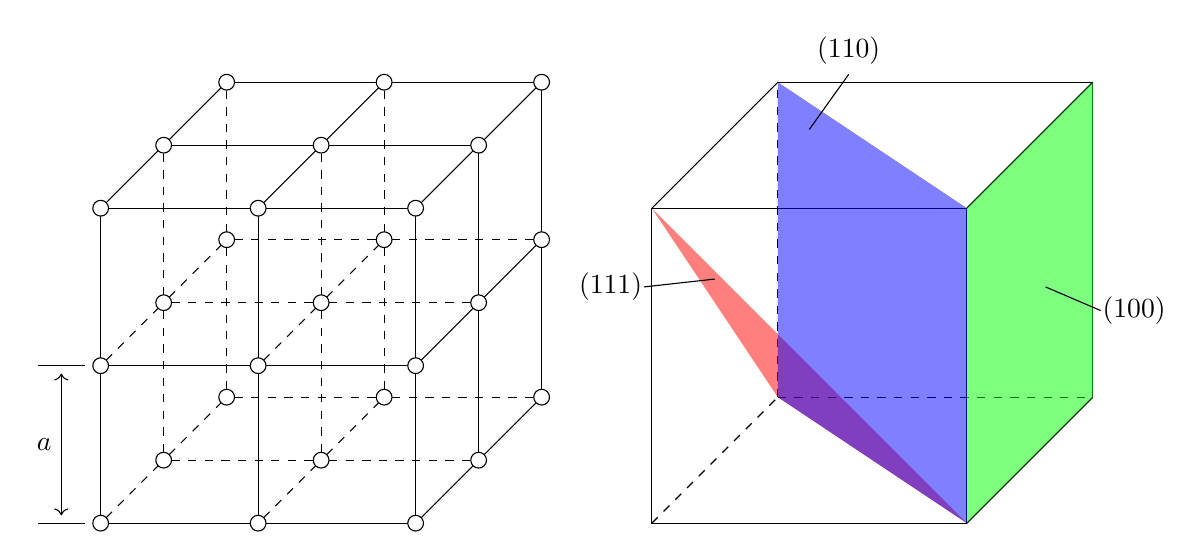
\begin{tikzpicture}
        \draw (0,0) circle [radius=0.1];
        \draw (2,0) circle [radius=0.1];
        \draw (4,0) circle [radius=0.1];
        \draw (4,2) circle [radius=0.1];
        \draw (4,4) circle [radius=0.1];
        \draw (0,2) circle [radius=0.1];
        \draw (0,4) circle [radius=0.1];
        \draw (2,2) circle [radius=0.1];
        \draw (2,4) circle [radius=0.1];
        \draw (0.8,0.8) circle [radius=0.1];
        \draw (0.8,2.8) circle [radius=0.1];
        \draw (0.8,4.8) circle [radius=0.1];
        \draw (2.8,0.8) circle [radius=0.1];
        \draw (4.8,0.8) circle [radius=0.1];
        \draw (2.8,2.8) circle [radius=0.1];
        \draw (2.8,4.8) circle [radius=0.1];
        \draw (4.8,2.8) circle [radius=0.1];
        \draw (4.8,4.8) circle [radius=0.1];				
        \draw (1.6,1.6) circle [radius=0.1];				
        \draw (3.6,1.6) circle [radius=0.1];				
        \draw (5.6,1.6) circle [radius=0.1];				
        \draw (1.6,3.6) circle [radius=0.1];				
        \draw (1.6,5.6) circle [radius=0.1];				
        \draw (3.6,3.6) circle [radius=0.1];				
        \draw (3.6,5.6) circle [radius=0.1];				
        \draw (5.6,3.6) circle [radius=0.1];				
        \draw (5.6,5.6) circle [radius=0.1];
        
        \draw (0.1,0)--(1.9,0);
        \draw (0,0.1)--(0,1.9);
        \draw (0,2.1)--(0,3.9);
        \draw (2.1,0)--(3.9,0);
        \draw (0.1,2)--(1.9,2);
        \draw (0.1,4)--(1.9,4);
        \draw (2.1,2)--(3.9,2);
        \draw (2.1,4)--(3.9,4);
        \draw (2,0.1)--(2,1.9);
        \draw (4,0.1)--(4,1.9);
        \draw (2,2.1)--(2,3.9);
        \draw (4,2.1)--(4,3.9);
        \draw [dashed] (0.8,0.9)--(0.8,2.7);
        \draw [dashed] (2.8,0.9)--(2.8,2.7);
        \draw (4.8,0.9)--(4.8,2.7);
        \draw [dashed] (0.9,0.8)--(2.7,0.8);
        \draw [dashed] (0.9,2.8)--(2.7,2.8);
        \draw (0.9,4.8)--(2.7,4.8);
        \draw [dashed] (0.8,2.9)--(0.8,4.7);
        \draw [dashed] (2.8,2.9)--(2.8,4.7);
        \draw (4.8,2.9)--(4.8,4.7);
        \draw [dashed] (2.9,0.8)--(4.7,0.8);
        \draw [dashed] (2.9,2.8)--(4.7,2.8);
        \draw (2.9,4.8)--(4.7,4.8);
        \draw [dashed] (1.6,1.7)--(1.6,3.5);
        \draw [dashed] (3.6,1.7)--(3.6,3.5);
        \draw (5.6,1.7)--(5.6,3.5);
        \draw [dashed] (1.6,3.7)--(1.6,5.5);
        \draw [dashed] (3.6,3.7)--(3.6,5.5);
        \draw (5.6,3.7)--(5.6,5.5);
        \draw [dashed] (1.7,1.6)--(3.5,1.6);
        \draw [dashed] (1.7,3.6)--(3.5,3.6);
        \draw (1.7,5.6)--(3.5,5.6);
        \draw [dashed] (3.7,1.6)--(5.5,1.6);
        \draw [dashed] (3.7,3.6)--(5.5,3.6);
        \draw (3.7,5.6)--(5.5,5.6);				
        \draw [dashed] (0.07,0.07)--(0.73,0.73);
        \draw [dashed] (0.07,2.07)--(0.73,2.73);
        \draw (0.07,4.07)--(0.73,4.73);				
        \draw [dashed] (2.07,0.07)--(2.73,0.73);
        \draw [dashed] (2.07,2.07)--(2.73,2.73);
        \draw (2.07,4.07)--(2.73,4.73);				
        \draw (4.07,0.07)--(4.73,0.73);
        \draw (4.07,2.07)--(4.73,2.73);
        \draw (4.07,4.07)--(4.73,4.73);				
        \draw [dashed] (0.87,0.87)--(1.53,1.53);
        \draw [dashed] (0.87,2.87)--(1.53,3.53);
        \draw (0.87,4.87)--(1.53,5.53);				
        \draw [dashed] (2.87,0.87)--(3.53,1.53);
        \draw [dashed] (2.87,2.87)--(3.53,3.53);
        \draw (2.87,4.87)--(3.53,5.53);				
        \draw (4.87,0.87)--(5.53,1.53);
        \draw (4.87,2.87)--(5.53,3.53);
        \draw (4.87,4.87)--(5.53,5.53);
        \draw (-0.2,0)--(-0.8,0);				
        \draw (-0.2,2)--(-0.8,2);
        \draw [<->](-0.5,0.1)--(-0.5,1.9);
        \node [left] at(-0.5,1) {$ a $};
        
        \draw (7,0) rectangle (11,4);
        \draw (7,4)--(8.6,5.6);
        \draw (11,4)--(12.6,5.6);
        \draw (8.6,5.6)--(12.6,5.6);
        \draw (11,0)--(12.6,1.6);
        \draw (12.6,1.6)--(12.6,5.6);
        \draw [dashed] (7,0)--(8.6,1.6);
        \draw [dashed] (8.6,1.6)--(8.6,5.6);
        \draw [dashed] (8.6,1.6)--(12.6,1.6);
        \fill [red,fill opacity=0.5] (8.6,1.6)--(7,4)--(11,0)--(8.6,1.6)--cycle;
        \fill [blue,fill opacity=0.5] (8.6,1.6)--(8.6,5.6)--(11,4)--(11,0)--cycle;
        \fill [green,fill opacity=0.5] (11,0)--(12.6,1.6)--(12.6,5.6)--(11,4)--(11,0)--cycle;
        \draw (6.9,3)--(7.8,3.1);
        \node [left] at(7,3) {(111)};
        \draw (9,5)--(9.5,5.7);
        \node [above] at(9.5,5.7) {(110)};
        \draw (12,3)--(12.7,2.7);
        \node [right] at(12.6,2.7) {(100)};
    \end{tikzpicture}
    \caption{立方晶格结构图}
    \label{fig-JingGe}
\end{figure}

晶体的组成原子或分子在空间内按照一定规律呈周期性排列。其中,最简单的结构之一是晶体中的原子沿着直角坐标系的 $x, y, z$ 三个方向,以固定的距离 $a$(晶格常数)进行周期性重复排列,从而形成简单的立方点阵。

可以将组成晶体的原子视为位于一系列相互平行且间距固定的平面族上,这些平面称为晶面。在晶面中,三种最为重要和常见的类型如图 \ref{fig-JingGe} 所示,分别为 (111) 面、(110) 面、(100) 面。括号中的三个数字称为晶面指数。晶面指数的一般确定方法如下:在右手系中,寻找该平面在 $x, y, z$ 轴上的截距 $x_0, y_0, z_0$,然后取其倒数并求比,即 $\frac{1}{x_0}:\frac{1}{y_0}:\frac{1}{z_0}$,将其化为最小整数比 $x_1 : y_1 : z_1$,那么该平面的晶面指数便为 $(x_1 y_1 z_1)$。

通常,对于晶面指数为 $(n_1 n_2 n_3)$ 的平面族,相邻两个晶面之间的距离为:
\[
d = \frac{a}{\sqrt{n_1^2 + n_2^2 + n_3^2}}
\]
\subsubsection{布拉格衍射}
\begin{figure}[!h]
    \centering
    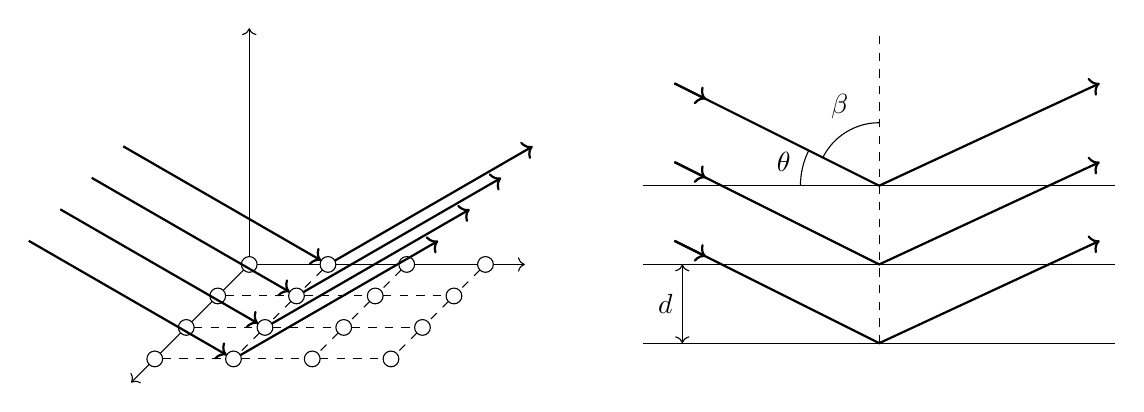
\begin{tikzpicture}
        \draw (-3,0)--(3,0);
        \draw (-3,2)--(3,2);
        \draw (-3,1)--(3,1);
        \draw [dashed] (0,0)--(0,4);
        \draw [<->] (-2.5,0)--(-2.5,1);
        \node [left] at(-2.5,0.5) {$ d $};
        \draw [thick,->] (-2.6,1.3)--(0,0)--(2.8,1.3);
        \draw [thick,->] (-2.6,1.3)--(-2.2,1.1);
        \draw [thick,->] (-2.6,2.3)--(0,1)--(2.8,2.3);
        \draw [thick,->] (-2.6,2.3)--(-2.2,2.1);
        \draw [thick,->] (-2.6,3.3)--(0,2)--(2.8,3.3);
        \draw [thick,->] (-2.6,3.3)--(-2.2,3.1);
        \draw (-1,2) arc (180:154:1);
        \draw (0,2.8) arc (90:154:0.8);
        \node [left] at(-1,2.3) {$\theta$};
        \node at(-0.5,3) {$\beta$};
        
        \draw (-8,1) circle [radius=0.1];
        \draw (-7,1) circle [radius=0.1];
        \draw (-6,1) circle [radius=0.1];
        \draw (-5,1) circle [radius=0.1];
        \draw (-8.4,0.6) circle [radius=0.1];
        \draw (-7.4,0.6) circle [radius=0.1];
        \draw (-6.4,0.6) circle [radius=0.1];
        \draw (-5.4,0.6) circle [radius=0.1];
        \draw (-8.8,0.2) circle [radius=0.1];
        \draw (-7.8,0.2) circle [radius=0.1];
        \draw (-6.8,0.2) circle [radius=0.1];
        \draw (-5.8,0.2) circle [radius=0.1];
        \draw (-9.2,-0.2) circle [radius=0.1];
        \draw (-7.2,-0.2) circle [radius=0.1];
        \draw (-8.2,-0.2) circle [radius=0.1];
        \draw (-6.2,-0.2) circle [radius=0.1];
        \draw [->] (-8,1.1)--(-8,4);
        \draw (-8.07,0.93)--(-8.33,0.67);
        \draw (-8.47,0.53)--(-8.73,0.27);
        \draw (-8.87,0.13)--(-9.13,-0.13);
        \draw [->] (-9.27,-0.27)--(-9.5,-0.5);
        \draw [dashed] (-7.07,0.93)--(-7.33,0.67);
        \draw [dashed] (-7.47,0.53)--(-7.73,0.27);
        \draw [dashed] (-7.87,0.13)--(-8.13,-0.13);
        \draw [dashed] (-6.07,0.93)--(-6.33,0.67);
        \draw [dashed] (-6.47,0.53)--(-6.73,0.27);
        \draw [dashed] (-6.87,0.13)--(-7.13,-0.13);
        \draw [dashed] (-5.07,0.93)--(-5.33,0.67);
        \draw [dashed] (-5.47,0.53)--(-5.73,0.27);
        \draw [dashed] (-5.87,0.13)--(-6.13,-0.13);
        \draw (-7.9,1)--(-7.1,1);
        \draw (-6.9,1)--(-6.1,1);
        \draw (-5.9,1)--(-5.1,1);
        \draw [->] (-4.9,1)--(-4.5,1);
        \draw [dashed] (-8.3,0.6)--(-7.5,0.6);
        \draw [dashed] (-7.3,0.6)--(-6.5,0.6);
        \draw [dashed] (-6.3,0.6)--(-5.5,0.6);
        \draw [dashed] (-8.7,0.2)--(-7.9,0.2);
        \draw [dashed] (-7.7,0.2)--(-6.9,0.2);
        \draw [dashed] (-6.7,0.2)--(-5.9,0.2);
        \draw [dashed] (-9.1,-0.2)--(-8.3,-0.2);
        \draw [dashed] (-8.1,-0.2)--(-7.3,-0.2);
        \draw [dashed] (-7.1,-0.2)--(-6.3,-0.2);
        \draw [thick,->] (-9.60,2.5)--(-7.086,1.05);
        \draw [thick,->] (-10.0,2.1)--(-7.486,0.65);
        \draw [thick,->] (-10.40,1.7)--(-7.886,0.25);
        \draw [thick,->] (-10.80,1.3)--(-8.286,-0.15);
        \draw [thick,->] (-6.91,1.05)--(-4.40,2.5);
        \draw [thick,->] (-7.31,0.65)--(-4.80,2.1);
        \draw [thick,->] (-7.71,0.25)--(-5.20,1.7);
        \draw [thick,->] (-8.11,-0.15)--(-5.60,1.3);
    \end{tikzpicture}
    \caption{同一晶面与不同晶面的散射波示意图}
    \label{fig-scatt}
\end{figure}
类似于光波在二维平面光栅上发生衍射,电磁波在进入晶体时同样会受到衍射作用。如果用三维空间中由原子构成的格点代替二维平面上的小孔,晶体则可以视作一个三维的光栅网络。晶体对电子波的衍射本质上是每个格点上的原子所产生的散射波的相干叠加。相干叠加的过程可以分为两步:第一步是同一晶面上各原子所发出的散射波相干叠加,从而形成该晶面的衍射波;第二步则是相同晶面族中相邻晶面之间的衍射波相干叠加。

位于同一个晶面上的原子共同产生的散射波,其相干叠加遵循反射定律。而从相隔 $d$ 的相邻两个晶面反射的波,其波程差为 $2d \sin \theta$,其中 $\theta$ 为入射角与晶面之间的夹角。显然,只有当满足以下条件时,才能形成干涉极大:
\[
2d \sin \theta = k \lambda, \qquad k = 1, 2, 3, \cdots
\]
此即为晶体衍射的布拉格条件。如果采用更常见的入射角 $\beta$ 来表示该条件,布拉格公式则可改写为:
\[
2d \cos \beta = k \lambda, \qquad k = 1, 2, 3, \cdots
\]
在本实验中,已知晶面间距 $d$,通过测量衍射极大时的入射角 $\beta$ 来确定波长 $\lambda$。

由于不同晶面族的几何取向不同、晶面间距也各不相同,当入射波的方向与波长固定,并且晶体取向也固定时,不同取向的晶面通常无法同时满足布拉格条件,有时甚至没有任何一族晶面能够满足这一条件。为了观察到尽可能多的衍射极大,并获得更多关于晶体结构的信息,实际的晶体结构研究中常采用以下方法:转动晶体、使用多晶或粉末样品替代单晶、以及使用包含连续波长的 X 射线代替固定波长的 X 射线。在本实验中,使用的是入射方向固定、单一波长的微波及单晶模型,因此通过转动晶体模型与调整接收喇叭的方向,来研究不同晶面的衍射现象。

\section{实验内容}
\subsection{实验前准备}
实验中所用微波频率一致,均为9.4\,GHz,打开电源后将微波频率设置为9.4\,GHz,并调整实验仪器在桌面上的位置与角度,使得检波器扫描范围能达到$ \pm50^\circ $。
同时,调节反射喇叭、接收喇叭、接受臂、活动臂为直线对齐状态,调节接收、发射喇叭高度相同。最后,对实验仪进行校准,确保发生器和接收器分别对准 $180^\circ$ 和 $0^\circ$ 位置,且接收信号在 $\pm 20^\circ$ 处的强度差在$2mV$以内。随后,调整微波发射功率,使得在零级极大点处接收到的信号强度大约在$120mV$到$150mV$之间。确保上述工作无误后开始实验。
\subsubsection{微波的双缝干涉实验}

根据实验要求,将双缝干涉板的缝宽均调节为 3.5\,cm。当将双缝干涉板固定于支座上时,应确保双缝板的平面与载物圆台上的 $90^\circ$ 指示线对齐。在 $-50^\circ \sim 50^\circ$ 的范围内,每隔 $2^\circ$ 读取一次液晶显示器的数值,并记录下测量数据,然后绘制出双缝干涉强度与角度的关系曲线。

在接近两侧的零级极大、零级极小及一级极小的位置,以 $1^\circ$ 为步长进行精细扫描。绘制精细扫描的结果曲线,以确定极值点的位置。

根据实验测得的微波干涉强度的零级极大、零级极小、一级极大的角度,以及双缝的缝宽 $a$ 和缝间间隔 $b$,计算微波的波长 $\lambda$ 及其百分误差。
\subsection{微波的迈克尔逊干涉实验}
利用微波的传播方向设置迈克尔逊干涉仪,并在极大位置适当调节微波发生器的输出功率,使接收信号的强度大于 100\,mV,以便清晰观察到信号强度的变化及极小值。当可移动反射板安装到旋转读数机构上后,通过操作旋转读数机构上的手柄移动反射板,测量出接收到的 $n+1$ 个微波干涉极小值的位置。同时,从读数机构上读取可移动反射板的移动距离 $L$,则微波的波长 $\lambda$ 满足以下关系:
\[
\lambda = \frac{2L}{n}
\]
\subsection{微波布拉格衍射实验}
\subsubsection{(100)晶面}
首先将发生器与检波器正对,并调节微波发生功率,使接收到的信号强度稳定在大约 $150\,\mathrm{mV}$ 左右。随后,安装模型晶体,并通过转动载物圆盘使发生器位于 $-30^\circ$(即 $330^\circ$)位置,同时将接收器旋转至 $30^\circ$,确保入射角和探测角相对于晶面法线对称。

在接下来测量过程中,调整入射角在 $30^\circ \sim 80^\circ$ 的范围内以 $2^\circ$ 为步长进行逐步步进,并在相应的探测位置读取和记录接收到的信号强度。根据测得的数据,绘制入射角与接收信号强度之间的关系图。

此外,在接近信号强度极大值点的位置,以 $1^\circ$ 为步长进行精确扫描,以确定对应的极大值点入射角。根据测得的极大值点入射角,计算微波的波长 $\lambda$,其表达式为:
\[
\lambda = 2d \cos \beta
\]
并进一步计算其百分误差。
\subsubsection{(110)晶面}
实验的主要步骤与 (100) 晶面时基本相同,但有所不同的是 (100) 晶面的晶面法线方向位于载物圆盘上的 $0^\circ$ 位置,而 (110) 晶面的晶面法线方向则位于载物圆盘上的 $45^\circ$ 位置。此外,在进行粗略扫描时,入射角的扫描范围应调整为 $30^\circ \sim 70^\circ$。在精细扫描过程中,由于接收信号较弱,可以适当调整微波发生器的功率,以确保信号的可观测性。

\section{实验结果与数据处理}
\subsection{实验前条件确认}
实验条件确认:微波频率9.4GHz\quad 微波波长3.1915cm
\begin{table}[!h]
    \centering
    \caption{微波实验仪对准确认}
    \begin{tabular}{|l|l|l|l|}
    \hline
        角度($^{\circ}$) & 0 & 20 & -20 \\ \hline
        电压(mV) & 131.6 & 8.3 & 8.0 \\ \hline
    \end{tabular}
\end{table}
由上表数据可知仪器基本已对准
\subsection{微波的双缝干涉实验}
实验所得数据如下表所示:
\newpage
\begin{table}[!h]
    \centering
    {\small(a)粗扫数据记录}
    \begin{tabularx}{\textwidth}{|c|Y|Y|Y|Y|Y|Y|Y|Y|Y|}
        \hline
        $ {\theta}\;(^\circ) $ & $ \bm 0 $ & $ \bm 2 $ & $ \bm 4 $ & $ \bm 6 $ & $ \bm 8 $ & $ \bm{10} $ & $ \bm{12} $ & $ \bm{14} $ & $ \bm{16} $\\
        \hline
        $ {U_{\theta+}}\;(\mathrm{mV}) $ & 29.4 & 27.8 & 22.9 & 13.8 & 2.0 & 0.2 & 0.0 & 0.2 & 2.0\\
        \hline
        $ U_{\theta-}\;(\mathrm{mV}) $ & 29.4 & 26.3 & 15.5 & 3.6 & 0.3 & 0.2 & 0.9 & 2.8 & 6.0\\
        \hline
        $ {\theta}\;(^\circ) $ & $ \bm{18} $ & $ \bm{20} $ & $ \bm{22} $ & $ \bm{24} $ & $ \bm{26} $ & $ \bm{28} $ & $ \bm{30} $ & $ \bm{32} $ & $ \bm{34} $\\
        \hline
        $ {U_{\theta+}}\;(\mathrm{mV}) $ & 6.3 & 11.2 & 16.5 & 17.1 & 8.8 & 2.6 & 1.0 & 0.5 & 0.4\\
        \hline
        $ U_{\theta-}\;(\mathrm{mV}) $ & 15.0 & 19.5 & 13.9 & 6.4 & 2.2 & 0.9 & 0.6 & 0.7 & 1.2\\
        \hline
        $ \theta\;(^\circ) $ & $ \bm{36} $ & $ \bm{38} $ & $ \bm{40} $ & $ \bm{42} $ & $ \bm{44} $ & $ \bm{46} $ & $ \bm{48} $ & $ \bm{50} $ &\\
        \hline
        $ {U_{\theta+}}\;(\mathrm{mV}) $ & 0.6 & 1.1 & 1.0 & 0.5 & 0.4 & 1.8 & 4.2 & 3.0 & \\
        \hline
        $ U_{\theta-}\;(\mathrm{mV}) $ & 1.5 & 1.0 & 0.2 & 0.6 & 2.8 & 5.1 & 2.3 & 0.2 & \\
        \hline
    \end{tabularx}

    ~\
    
    {\small(b)正负侧一级极大处细扫数据}\\
    \begin{tabularx}{\textwidth}{|c|c|Y|Y|Y|Y|Y|Y|Y|Y|Y|}
        \hline
        \multirow{4}*{一级极大} & $ \theta\;(^\circ) $ & $ \bm{20} $ & $ \bm{21} $ & $ \bm{22} $ & $ \bm{23} $ & $ \bm{24} $ & $ \bm{25} $ & $ \bm{26} $ & $ \bm{27} $ & $ \bm{28} $\\
        \cline{2-11}
        & $ U_{\theta+}\;(\mathrm{mV}) $ & 11.5 & 14.0 & 17.1 & 17.2 & 17.5 & 13.9 & 9.4 & 6.1 & 2.7\\
        \cline{2-11}
        & $ \theta\;(^\circ) $ & $ \bm{16} $ & $ \bm{17} $ & $ \bm{18} $ & $ \bm{19} $ & $ \bm{20} $ & $ \bm{21} $ & $ \bm{22} $ & $ \bm{23} $ & $ \bm{24} $\\
        \cline{2-11}
        & $ U_{\theta-}\;(\mathrm{mV}) $ & 6.2 & 10.7 & 15.1 & 18.3 & 19.5 & 18.1 & 14.1 & 9.7 & 6.4\\
        \hline
    \end{tabularx}
            
    ~\
    
    {\small(c)正负侧零级极小处细扫数据}\\
    \begin{tabularx}{\textwidth}{|c|c|Y|Y|Y|Y|Y|Y|Y|Y|Y|}
        \hline
        \multirow{4}*{零级极小} & $ \theta\;(^\circ) $ & $ \bm{8} $ & $ \bm{9} $ & $ \bm{10} $ & $ \bm{11} $ & $ \bm{12} $ & $ \bm{13} $ & $ \bm{14} $ & $ \bm{15} $ & $ \bm{16} $\\
        \cline{2-11}
        & $ U_{\theta+}\;(\mathrm{mV}) $ & 2.0 & 1.0 & 0.2 & 0.1 & 0.0 & 0.1 & 0.2 & 1.0 & 2.0\\
        \cline{2-11}
        & $ \theta\;(^\circ) $ & $ \bm{6} $ & $ \bm{7} $ & $ \bm{8} $ & $ \bm{9} $ & $ \bm{10} $ & $ \bm{11} $ & $ \bm{12} $ & $ \bm{13} $ & $ \bm{14} $\\
        \cline{2-11}
        & $ U_{\theta-}\;(\mathrm{mV}) $ & 3.9 & 1.1 & 0.3 & 0.2 & 0.3 & 0.6 & 1.2 & 2.0 & 2.8\\
        \hline
    \end{tabularx}
    
    ~\
    
    {\small(d)正负侧一级极小处细扫数据}\\
    \begin{tabularx}{\textwidth}{|c|c|Y|Y|Y|Y|Y|Y|Y|Y|Y|}
        \hline
        \multirow{4}*{一级极小} & $ \theta\;(^\circ) $ & $ \bm{30} $ & $ \bm{31} $ & $ \bm{32} $ & $ \bm{33} $ & $ \bm{34} $ & $ \bm{35} $ & $ \bm{36} $ & $ \bm{37} $ & $ \bm{38} $\\
        \cline{2-11}
        & $ U_{\theta+}\;(\mathrm{mV}) $ & 1.3 & 0.7 & 0.5 & 0.4 & 0.4 & 0.5 & 0.6 & 0.8 & 1.1\\
        \cline{2-11}
        & $ \theta\;(^\circ) $ & $ \bm{26} $ & $ \bm{27} $ & $ \bm{28} $ & $ \bm{29} $ & $ \bm{30} $ & $ \bm{31} $ & $ \bm{32} $ & $ \bm{33} $ & $ \bm{34} $\\
        \cline{2-11}
        & $ U_{\theta-}\;(\mathrm{mV}) $ & 2.3 & 1.4 & 0.9 & 0.7 & 0.7 & 0.7 & 0.8 & 0.9 & 1.2\\
        \hline
    \end{tabularx}
    \caption{微波双缝干涉数据记录表}
\end{table}
根据上表数据绘图,得到如下图像:
\newpage
\begin{figure}[!h]
    \centering
    \includegraphics*[scale=0.1]{fig2.jpg}
    \caption{双缝干涉实验数据图像}
\end{figure}
观察粗扫图像,图像整体呈现出较好的对称性,并且在接近 $0^\circ$ 处观察到干涉极大,符合理论预期。粗略估计,一级极大约出现在 $23^\circ$ 附近,零级极小大约在 $12^\circ$ 附近,一级极小大概位于 $33^\circ$ 附近。接下来将围绕这些角度进行精细扫描。

然而,实验数据与理论值之间存在一定的偏差。实验中测得的零级极大并未严格出现在 $0^\circ$ 角处,且正负角度的图像并非完全对称,存在一定偏移。导致这些误差的潜在原因可能包括:
在读数过程中,仪器无法提供稳定的数值,指示读数存在小幅波动,数值读取存在主观性;
在实验前的校准过程中,实验仪器未能完全对正,尤其是在正负 $20^\circ$时仪器读数并不完全相同。这可能导致初始位置的零点发生偏移;
实验中的双缝板可能存在一定的缺陷,导致实际的双缝宽度与实验中设定的宽度存在一定的偏差;
实验过程中可能无意中触碰了实验台,导致初始的仪器对准遭到破坏。 

观察正负一级极大细扫图像,通过取两图中峰值对应角度的绝对值的平均数,可以有效消除由于零点偏移带来的误差。计算得出一级极大对应的角度为 $\theta_0 = 22.0^{\circ}$。将该值代入公式来计算微波的波长,得到:
\[
\lambda = (a + b) \sin \theta_0 = 3.184\, \mathrm{cm}
\]
其相对误差为 $0.188\%$,较好的吻合了实际的波长数值。

观察正负零级极小细扫图像,通过对两图中峰值对应角度的绝对值求平均,可以消除角度零点偏移的影响。计算得出零级极小对应的角度为 $\theta_0 = 10。5^{\circ}$。将其代入公式,计算得到微波的波长为:
\[
\lambda = 2(a + b) \sin \theta_0 = 3.098\, \mathrm{cm}
\]
相对误差为 $2.88\%$,产生了相对较大的误差。

观察正负一级极小细扫图像,通过对两图中极小值对应角度的绝对值求取平均,可以有效消除零点偏移。计算得出的一级极小对应的角度为 $\theta_0 = 31.75^\circ$。将该角度代入公式,得到微波波长为:
\[
\lambda = \frac{2}{3}(a + b) \sin \theta_0 = 2.982\, \mathrm{cm}
\]
相对误差为 $6.52\%$,与理论值相比存在较大的误差。

\subsection{微波的迈克尔逊干涉实验}
实验所得数据如下表所示:
\begin{table}[!h]
    \centering
    \begin{tabularx}{\textwidth}{|c|Y|Y|Y|Y|}
        \hline
        最小点读数(cm) & 6.65 & 5.05 & 3.45 & 1.89\\
        \hline
    \end{tabularx}
    \caption{迈克尔逊干涉实验数据记录表}
\end{table}
用逐差法处理数据,选取第 1、2 个极小作为一组,第 1、3 个极小作为一组,第 1、4 个极小作为一组,分别计算得到微波波长为:
\[
\lambda_1 = \frac{2L}{1} = 3.20\,\mathrm{cm}, \quad \lambda_2 = \frac{2L}{2} = 3.20\,\mathrm{cm}, \quad \lambda_3 = \frac{2L}{3} = 3.17\,\mathrm{cm}
\]
取其平均值作为测量结果,得到
\[
\bar{\lambda} = 3.19\,\mathrm{cm}
\]
平均结果完全符合实际波长数据。
\subsection{微波布拉格衍射实验}
\subsubsection{(100)晶面}
实验所得数据如下表所示:
\newpage
\begin{table}[!h]
    \centering
    {\small(a)粗扫数据记录}
    \begin{tabularx}{\textwidth}{|c|Y|Y|Y|Y|Y|Y|Y|Y|Y|}
        \hline
        $ \varphi_{\mathrm{I}}\;(^\circ) $ & $ \bm{30} $ & $ \bm{32} $ & $ \bm{34} $ & $ \bm{36} $ & $ \bm{38} $ & $ \bm{40} $ & $ \bm{42} $ & $ \bm{44} $ & $ \bm{46} $\\
        \hline
        $ U\;(\mathrm{mV}) $ & 1.8 & 2.1 & 1.7 & 1.7 & 2.21 & 3.6 & 3.4 & 0.8 & 0.4\\
        \hline
        $ \varphi_{\mathrm{I}}\;(^\circ) $ & $ \bm{48} $ & $ \bm{50} $ & $ \bm{52} $ & $ \bm{54} $ & $ \bm{56} $ & $ \bm{58} $ & $ \bm{60} $ & $ \bm{62} $ & $ \bm{64} $\\
        \hline
        $ U\;(\mathrm{mV}) $ & 3.0 & 5.2 & 1.3 & 0.5 & 1.5 & 1.5 & 7.0 & 20.0 & 12.8\\
        \hline
        $ \varphi_{\mathrm{I}}\;(^\circ) $ & $ \bm{66} $ & $ \bm{68} $ & $ \bm{70} $ & $ \bm{72} $ & $ \bm{74} $ & $ \bm{76} $ & $ \bm{78} $ & $ \bm{80} $ &\\
        \hline
        $ U\;(\mathrm{mV}) $ & 46.7 & 81.4 & 28.7 & 1.7 & 3.3 & 9.5 & 0.0 & 3.4 &\\
        \hline
    \end{tabularx}

~\

    {\small(b)极大值点附近细扫结果}
    \begin{tabularx}{\textwidth}{|c|Y|Y|Y|Y|Y|Y|Y|Y|Y|}
        \hline
        $ \varphi_{\mathrm{I}}\;(^\circ) $ & $ \bm{64} $ & $ \bm{65} $ & $ \bm{66} $ & $ \bm{67} $ & $ \bm{68} $ & $ \bm{69} $ & $ \bm{70} $ & $ \bm{71} $ & $ \bm{72} $\\
        \hline
        $ U\;(\mathrm{mV}) $ & 12.8 & 19.5 & 46.7 & 59.7 & 81.4 & 80.1 & 32.2 & 2.2 & 1.7\\
        \hline
    \end{tabularx}
    \caption{(100)晶面布拉格衍射数据记录表}
\end{table}
根据上表数据绘图,得到如下图像:
\begin{figure}[!h]
    \centering
    \includegraphics*[scale=0.15]{fig3.jpg}
    \caption{(100)晶面布拉格衍射实验数据图像}
\end{figure}

在100晶面中,面间距$d=4cm$,且根据实验数据可知,衍射极大值出现在$ \beta=68^\circ $处,
计算得到波长为$ \lambda=2d\cos\beta=3.00\,\mathrm{cm} $,相对误差为$ 5.96\% $,与实际波长值存在一定误差。

\subsubsection{(110)晶面}
实验所得数据如下表所示:
\newpage
\begin{table}[!h]
    \centering
    {\small(a)粗扫数据记录}
    \begin{tabularx}{\textwidth}{|c|Y|Y|Y|Y|Y|Y|Y|Y|Y|}
        \hline
        $ \varphi_{\mathrm{I}}\;(^\circ) $ & $ \bm{30} $ & $ \bm{32} $ & $ \bm{34} $ & $ \bm{36} $ & $ \bm{38} $ & $ \bm{40} $ & $ \bm{42} $ & $ \bm{44} $ & $ \bm{46} $\\
        \hline
        $ U\;(\mathrm{mV}) $ & 0.1 & 0.3 & 0.2 & 0.4 & 0.2 & 0.4 & 0.3 & 0.8 & 2.7\\
        \hline
        $ \varphi_{\mathrm{I}}\;(^\circ) $ & $ \bm{48} $ & $ \bm{50} $ & $ \bm{52} $ & $ \bm{54} $ & $ \bm{56} $ & $ \bm{58} $ & $ \bm{60} $ & $ \bm{62} $ & $ \bm{64} $\\
        \hline
        $ U\;(\mathrm{mV}) $ & 3.7 & 8.0 & 28.0 & 47.8 & 36.5 & 37.9 & 29.3 & 0.9 & 2.8\\
        \hline
        $ \varphi_{\mathrm{I}}\;(^\circ) $ & $ \bm{66} $ & $ \bm{68} $ & $ \bm{70} $ & &&&&&\\
        \hline
        $ U\;(\mathrm{mV}) $ & 0.5 & 0.1 & 0.1 & &&&&&\\
        \hline
    \end{tabularx}

~\

    {\small(b)极大值点附近细扫结果}
    \begin{tabularx}{\textwidth}{|c|Y|Y|Y|Y|Y|Y|Y|Y|Y|}
        \hline
        $ \varphi_{\mathrm{I}}\;(^\circ) $ & $ \bm{50} $ & $ \bm{51} $ & $ \bm{52} $ & $ \bm{53} $ & $ \bm{54} $ & $ \bm{55} $ & $ \bm{56} $ & $ \bm{57} $ & $ \bm{58} $\\
        \hline
        $ U\;(\mathrm{mV}) $ & 7.8 & 16.9 & 27.3 & 35.3 & 46.8 & 49 & 36.5 & 34.1 & 36.5\\
        \hline
    \end{tabularx}
\caption{(110)晶面布拉格衍射数据记录表}
\end{table}
根据上表数据绘图,得到如下图像:
\begin{figure}[!h]
    \centering
    \includegraphics*[scale=0.16]{fig4.jpg}
    \caption{(110)晶面布拉格衍射实验数据图像}
\end{figure}

在100晶面中,面间距$d=2\sqrt{2}cm$,且根据实验数据可知,衍射极大值出现在$ \beta=55^\circ $处,
计算得到波长为$ \lambda=2d\cos\beta=3.24\,\mathrm{cm} $,相对误差为$ 1.57\% $,与实际波长值存在较小误差。

\section{讲义思考题}
\subsection{各实验中误差的主要影响是什么}
\textit{在实验进行过程中,若接收喇叭与发射喇叭未能完全对齐,使得接收信号在 $0^\circ$ 处未能达到最大值,或是在初始实验条件校准时正负$20^\circ$处的信号强度相差较大,则测得的数据和绘制的图像将表现出相对于 $\theta=0^\circ$ 明显的不对称性。这种偏差会在细致扫描治疗得到峰值时更加显著,正负两侧获得的峰值角度可能有较大的差距。这种情况会导致计算微波波长时产生一定误差。实际上,在实验中很难让 $\pm 20^\circ$ 收到的信号强度完全一致(即使做到,也是局限于实验仪器的精度范围内)。因此,实验所得数据不可避免会在横坐标方向有所偏移,适当校准仪器,减小这种偏移,将能提高实验结果的准确性。}

\textit{除了上述情况外,每个实验还存在一些通用的误差来源,例如接收喇叭的精度限制以及角度测量时的误差。前者主要表现在实验 1 的极小值附近——在极小值的位置,粗略扫描的数据可能显示为多个 $0.0\, \mathrm{mV}$。若在精细扫描时未能调节微波强度至一个恰当的数值,这将导致若干个 $0$ 值影响对极小值点的准确确定。后者则体现在调节接收臂至指定角度时,有时无法精确对准角度,从而导致部分数据点的测量值有较大的偏差。同时,实验仪器在测量负角度一侧的数据时,若接收臂未予以固定,就会向逆时针滑动,无法准确读取目标角度的数据;而当手动固定接收臂时,很难确保读数过程中是否由于不经意造成接收臂角度的偏移,导致测量误差。}

\textit{在双缝干涉实验中,缝宽和缝间的间隔存在误差,且衍射板不可能严格垂直于微波传播方向,这些都将引发实验结果与理论值的偏离。}

\textit{在迈克尔逊干涉实验中,反射板与玻璃板实际摆放时的角度偏差同样会对实验结果的准确性构成影响。为了避免由于回程差导致的误差,粗调可移动反射板时应始终沿一个方向移动,并从初始位置开始逐一测量各极小点。}

\textit{在微波布拉格衍射实验中,晶体模型的排列方式以及尼龙绳对小球的固定都会对实验数据产生干扰。尽管在实验前会对小球间距进行调整,但仍无法保证每个小球之间的间隔都严格等于$4cm$}

\subsection{金属是一种良好的微波反射器。其它物质的反射特性如何?是否有部分能量透过这些物质还是被吸收了?比较导体与非导体的反射特性。}
\textit{金属作为良好的微波反射器,其反射特性源于金属内的自由电子对电磁波的响应。在电磁波作用下,金属表面产生强烈的感应电流,阻止电磁波进一步进入材料,因而将大部分的能量反射回去。然而,材料的反射、透射和吸收行为在很大程度上取决于它们的导电性、介电常数和磁导率。}

\textit{相较而言,导体与非导体在电磁波的互动上存在显著的差异。导体(如金属)由于具有高度的自由电子密度,其电磁反射性能较强,通常对微波或更高频率的电波具有高反射性和低透射性,而只有极少部分能量被吸收,通常吸收主要发生在非常薄的表面层,称为“趋肤效应”。而非导体(如绝缘体或介电材料),由于电子无法自由运动,电磁波可以部分透过这些材料。介电材料在此类电磁波频率下的反射性通常较弱,具体的透射与反射比例取决于其介电常数和损耗因子。部分能量可能被吸收,这取决于材料的损耗机制,如介电损耗或磁损耗。}

\textit{因此,总体来看,导体具有极高的反射性且吸收能量极少,而非导体具有较低的反射性且透射性更高,同时会伴随一定程度的能量吸收。}

\subsection{为避免每台仪器微波间的干扰,使用吸波材料对每套设备进行了微波屏蔽,请问吸波材料的工作机理是什么?与屏蔽微波波长的关系是什么?}
\textit{海绵吸波材料在实验中的应用旨在减少和防止各组实验仪器之间的互相干扰,其工作原理基于将入射到材料表面的微波通过多种物理机制进行吸收和衰减,从而避免反射和接近设备的微波源对外部进行泄露。吸波材料通常采用具有高介电损耗或高磁损耗的材料,其内部结构使得微波在进入材料后逐渐耗散为热能。一个关键的机制是通过材料内的电磁波阻抗匹配和产生多次反射,使得电磁波在内部经历逐步衰减,最终能量耗散为不可测的热量,以避免从材料表面返回的反射能量。}

\textit{吸波材料的有效性与微波波长密切相关。为了增强材料对特定波长微波的吸收效果,通常将材料的厚度设计为波长的某个比例,使得入射微波在材料内部产生长度相应的衰减路径,通过多层结构的干涉效应和材料的损耗特性,最大限度地提高吸收率。通常,吸波材料针对特定频率或波长的微波具有优化的设计,因此使用时应确保材料的吸波性能与微波频率匹配,以达到最佳的屏蔽效果。}

\subsection{假如预先不知道晶体中晶面的方向,是否会增加实验的复杂性?又该如何定位这些晶面?}
\textit{在预先不知道晶体中晶面方向的情况下,实验的复杂性会增加。实验的复杂性主要来自于不确定晶体的特定晶面如何与入射波发生相互作用。为了克服这一复杂性,实验可以通过一种迭代的方式进行。首先,固定晶体与入射波之间的夹角,即入射角,然后改变接收臂的角度,通过观察接收信号的变化来寻找信号的极大值点。当接收到的信号达到峰值时,意味着发生了显著的反射现象,此时的接收角度就是反射角。根据布拉格定律$$2d\sin\theta=n\lambda$$,其中$d$为晶面间距,$\theta$为入射角,$n$为整数,$\lambda$为波长,已知波长$\lambda$,通过测量反射角$\theta$,可以进一步计算出晶面间距$d$,从而推测晶面的方向。}

\end{document}